\documentclass[11pt]{beamer}
\usetheme{CambridgeUS}
\usepackage[utf8]{inputenc}
\usepackage{amsmath}
\usepackage{amsfonts}
\usepackage{amssymb}
\usepackage{graphicx}
\usepackage{pgfpages}
\usepackage{framed}
\usepackage{xcolor}
\usepackage[most]{tcolorbox}
\usepackage{soul}
\usepackage{empheq}

% The replacement character � (often displayed as a black rhombus with a white
% question mark) is a symbol found in the Unicode standard at code point U
% +FFFD in the Specials table. It is used to indicate problems when a system 
% is unable to render a stream of data to a correct symbol.[4] It is usually 
% seen when the data is invalid and does not match any character. For this 
% reason we map explicitly this character to a blanck space.
\DeclareUnicodeCharacter{FFFD}{ }

\newcommand*{\itemimg}[1]{%
  \raisebox{-.3\baselineskip}{%
    \includegraphics[
      height=\baselineskip,
      width=\baselineskip,
      keepaspectratio,
    ]{#1}%
  }%
}

\newtcbox{\mymath}[1][]{%
    nobeforeafter, math upper, tcbox raise base,
    enhanced, colframe=blue!30!black,
    colback=blue!10, boxrule=1pt,
    #1}

\newcommand{\hlym}[1]{%
  \colorbox{yellow!100}{$\displaystyle#1$}}

\newcommand{\hlgm}[1]{%
  \colorbox{green!100}{$\displaystyle#1$}}

\newcommand{\hly}[1]{\colorbox{yellow!100}{#1}}

\newcommand{\hlg}[1]{\colorbox{green!100}{#1}}

\author{Giovanni Della Lunga\\{\footnotesize giovanni.dellalunga@unibo.it}}
%\title{1.1 - Introduction to Machine Learning}
\title{1.2 - Data Gathering with Pandas}
%\title{2.1 - Data Pre-Processing}
%\title{4.1 - Linear and Logistic Regression}
%\title{4.2 - Decision Trees}
%\title{6 - Text Vectorization}
%\title{7 - Classification for Text Analysis}
%\title{8 - Clustering for Text Similarity}
%\title{9 - Information Extraction}
\subtitle{} % (optional)
\setbeamercovered{transparent} 
\institute{Introduction to Machine Learning for Finance} 
\date{Bologna - February-March, 2025} 

\begin{document}

%\begin{frame}
%\includegraphics[width=\linewidth]{img/halloween-seminar-logo.PNG}
%\end{frame}

\begin{frame}
\titlepage
\end{frame}

\AtBeginSection[]
{
  %\begin{frame}<beamer>
  %\footnotesize	
  %\frametitle{Outline}
  %\begin{multicols}{2}
  %\tableofcontents[currentsection]
  %\end{multicols}	  
  %\normalsize
  %\end{frame}
  \begin{frame}
  \vfill
  \centering
  \begin{beamercolorbox}[sep=8pt,center,shadow=true,rounded=true]{title}  	\usebeamerfont{title}\insertsectionhead\par%
  \end{beamercolorbox}
  \vfill
  \end{frame}
}
\AtBeginSubsection{\frame{\subsectionpage}}

% INSERT HERE
%===================================================================================================
\section{Financial Data Gathering using Pandas \\ \scalebox{0.8}{}}
%---------------------------------------------------------------------------------------------------
\subsection{Pandas Datareader \\ \scalebox{0.8}{}}
%---------------------------------------------------------------------------------------------------
\begin{frame}{Data Gathering with Pandas}
	\begin{center}
	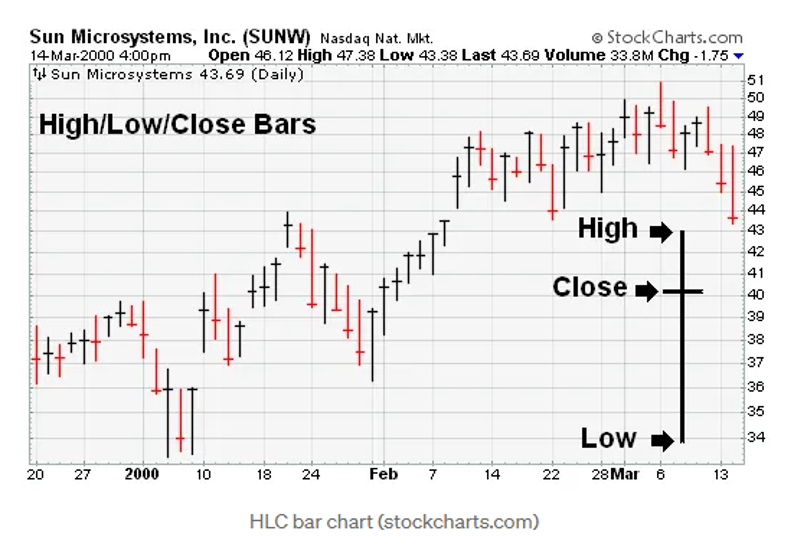
\includegraphics[scale=0.55]{../05-pictures/lesson-1-3_pic_0.png}
	\end{center}
\end{frame}
%..................................................................
\begin{frame}{Data Gathering with Pandas}
	\begin{center}
	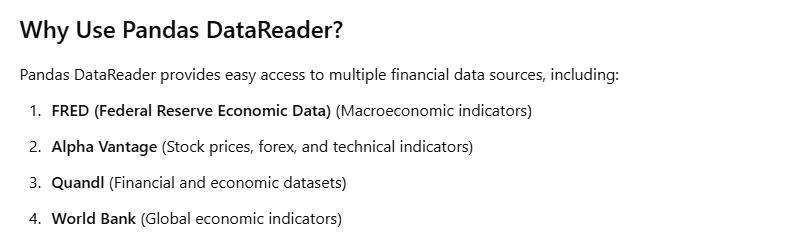
\includegraphics[scale=0.55]{../05-pictures/lesson-1-3_pic_1.png}
	\end{center}
\end{frame}
%..................................................................
\begin{frame}{Data Gathering with Pandas}
	\begin{center}
	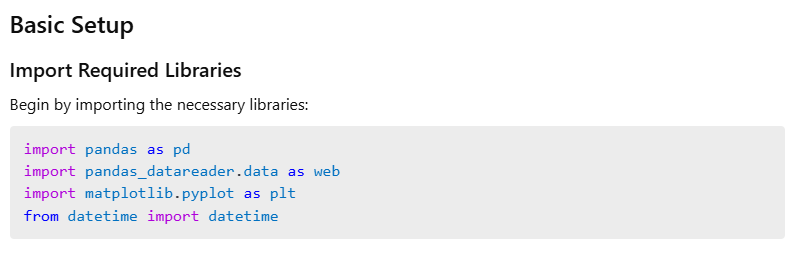
\includegraphics[scale=0.55]{../05-pictures/lesson-1-3_pic_2.png}
	\end{center}
\end{frame}
%..................................................................
\begin{frame}{Data Gathering with Pandas}
	\begin{center}
	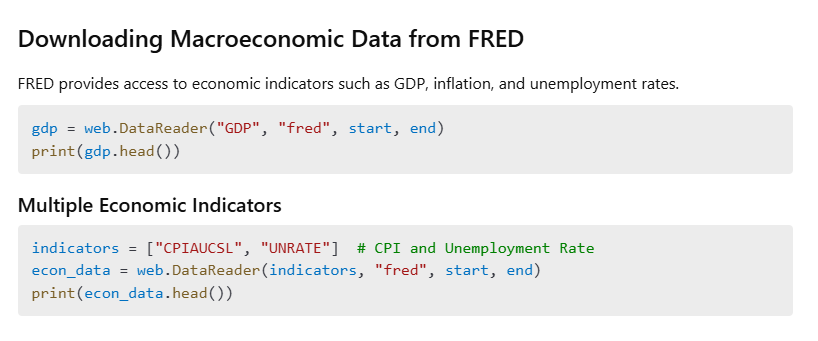
\includegraphics[scale=0.55]{../05-pictures/lesson-1-3_pic_3.png}
	\end{center}
\end{frame}
%..................................................................
\begin{frame}{Data Gathering with Pandas}
	\begin{center}
	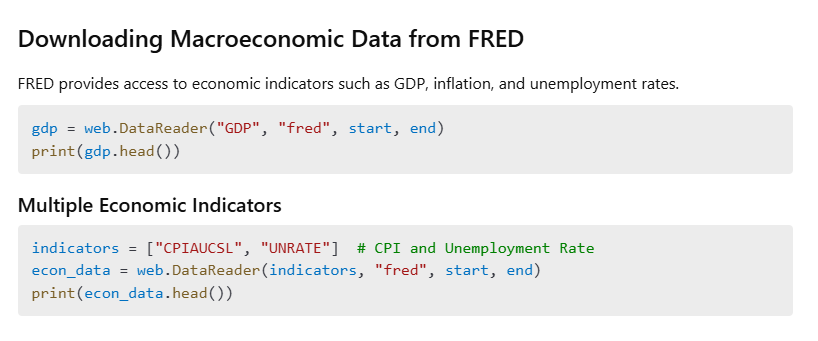
\includegraphics[scale=0.55]{../05-pictures/lesson-1-3_pic_4.png}
	\end{center}
\end{frame}
%..................................................................
\begin{frame}{Data Gathering with Pandas}
	\begin{center}
	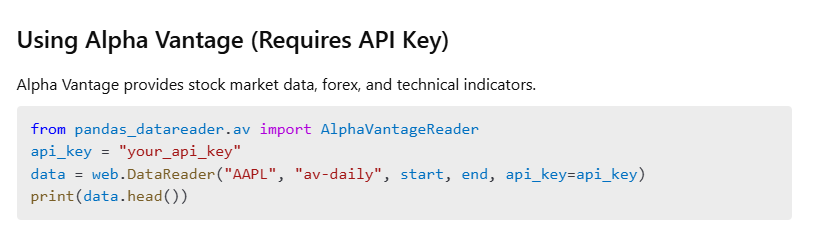
\includegraphics[scale=0.55]{../05-pictures/lesson-1-3_pic_5.png}
	\end{center}
\end{frame}
%..................................................................
\begin{frame}{Data Gathering with Pandas}
	\begin{center}
	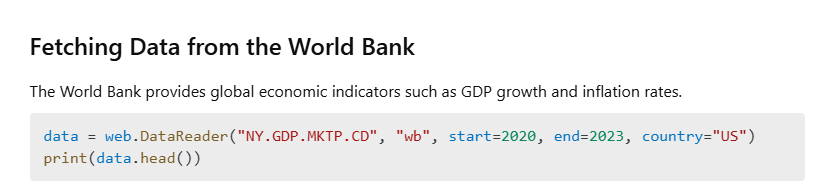
\includegraphics[scale=0.55]{../05-pictures/lesson-1-3_pic_6.png}
	\end{center}
\end{frame}
%..................................................................
\begin{frame}{Data Gathering with Pandas}
	\begin{center}
	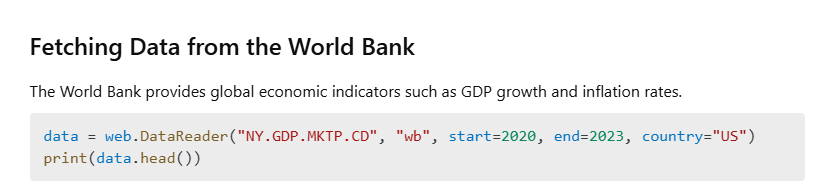
\includegraphics[scale=0.55]{../05-pictures/lesson-1-3_pic_7.png}
	\end{center}
\end{frame}
%..................................................................
\begin{frame}{Data Gathering with Pandas}
	\begin{center}
	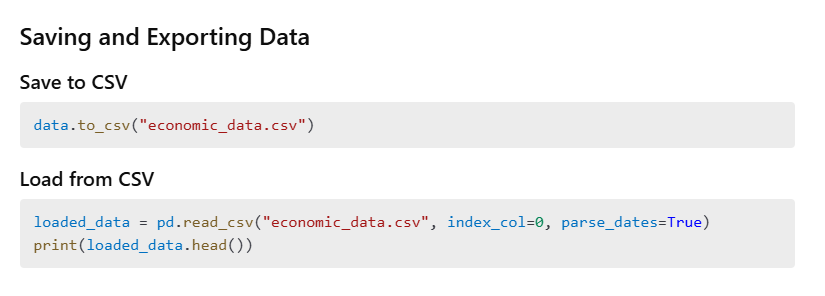
\includegraphics[scale=0.55]{../05-pictures/lesson-1-3_pic_8.png}
	\end{center}
\end{frame}
%..................................................................
\subsection{Yahoo Finance \\ \scalebox{0.8}{Using the yfinance python library}}
%---------------------------------------------------------------------------------------------------
\begin{frame}{Data Gathering with Pandas}
	\begin{center}
	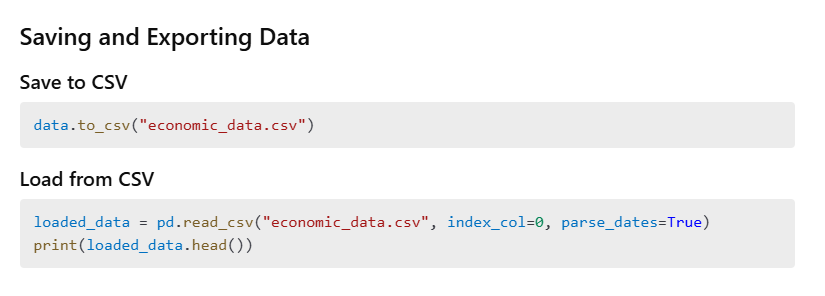
\includegraphics[scale=0.55]{../05-pictures/lesson-1-3_pic_9.png}
	\end{center}
\end{frame}
%..................................................................
\begin{frame}{Data Gathering with Pandas}
	\begin{center}
	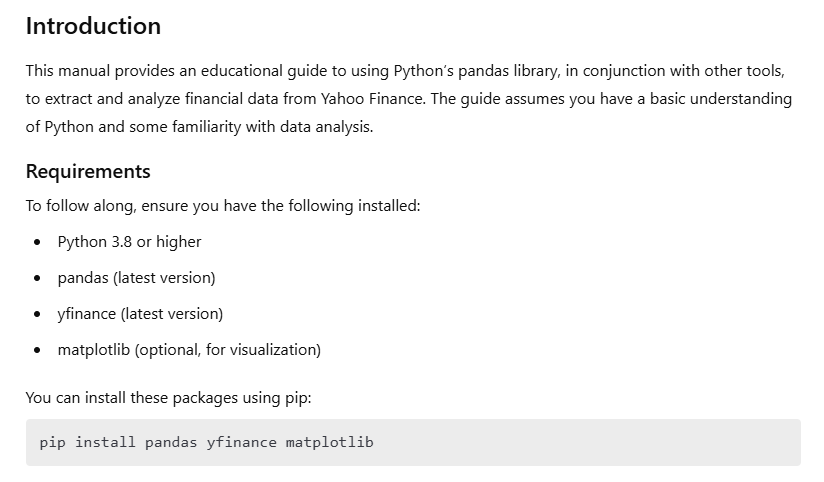
\includegraphics[scale=0.55]{../05-pictures/lesson-1-3_pic_10.png}
	\end{center}
\end{frame}
%..................................................................
\begin{frame}{Data Gathering with Pandas}
	\begin{center}
	
\includegraphics[scale=0.55]{../05-pictures/lesson-1-3_pic_11.png}
	\end{center}
\end{frame}
%..................................................................
\begin{frame}{Data Gathering with Pandas}
	\begin{center}
	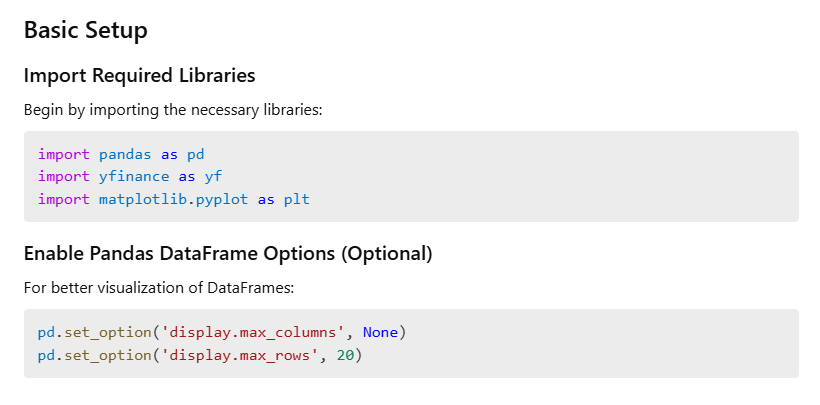
\includegraphics[scale=0.55]{../05-pictures/lesson-1-3_pic_12.png}
	\end{center}
\end{frame}
%..................................................................
\begin{frame}{Data Gathering with Pandas}
	\begin{center}
	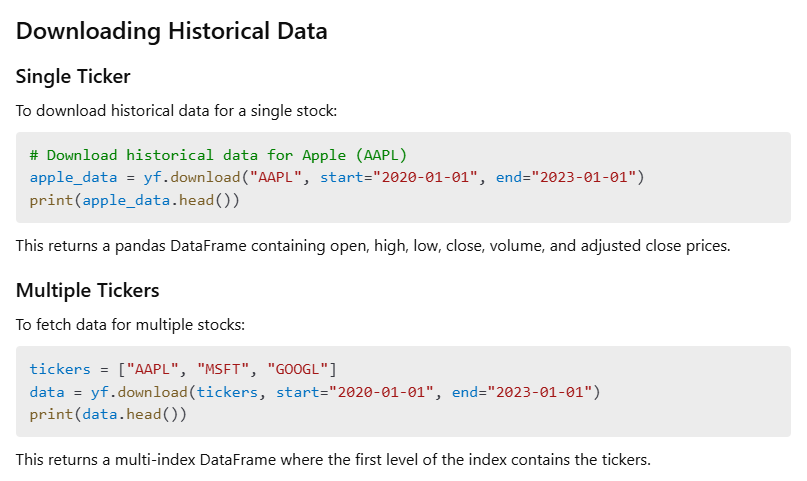
\includegraphics[scale=0.55]{../05-pictures/lesson-1-3_pic_13.png}
	\end{center}
\end{frame}
%..................................................................
\begin{frame}{Data Gathering with Pandas}
	\begin{center}
	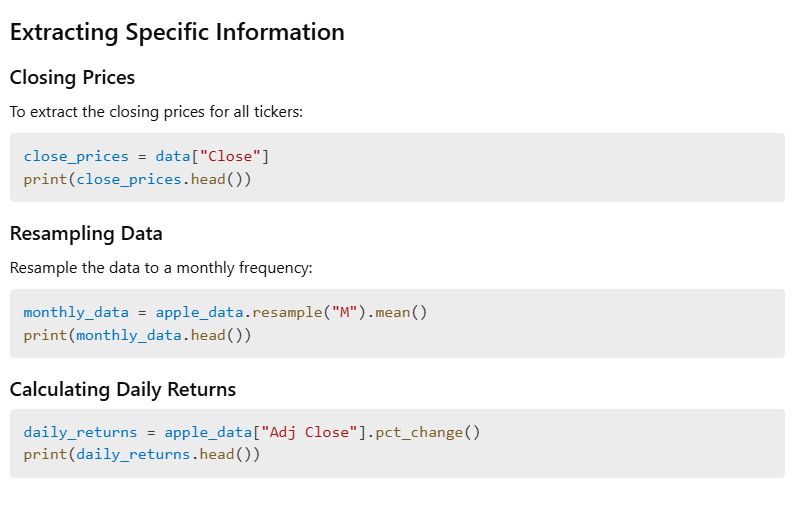
\includegraphics[scale=0.55]{../05-pictures/lesson-1-3_pic_14.png}
	\end{center}
\end{frame}
%..................................................................
\begin{frame}{Data Gathering with Pandas}
	\begin{center}
	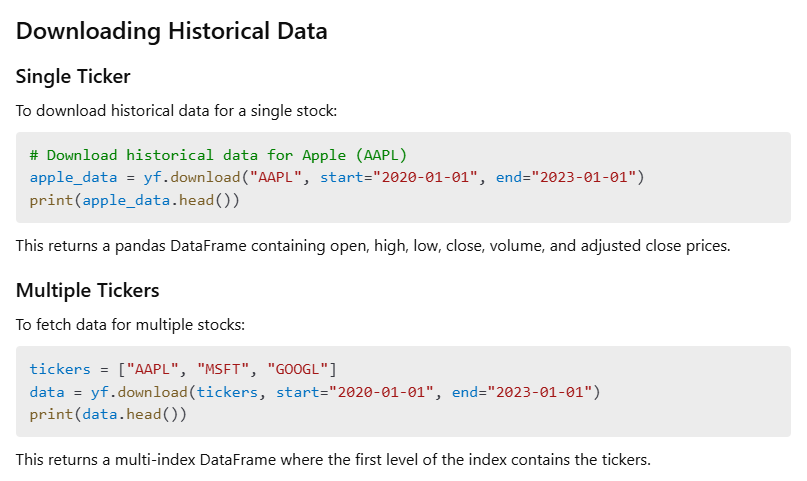
\includegraphics[scale=0.55]{../05-pictures/lesson-1-3_pic_15.png}
	\end{center}
\end{frame}
%..................................................................
\begin{frame}{Data Gathering with Pandas}
	\begin{center}
	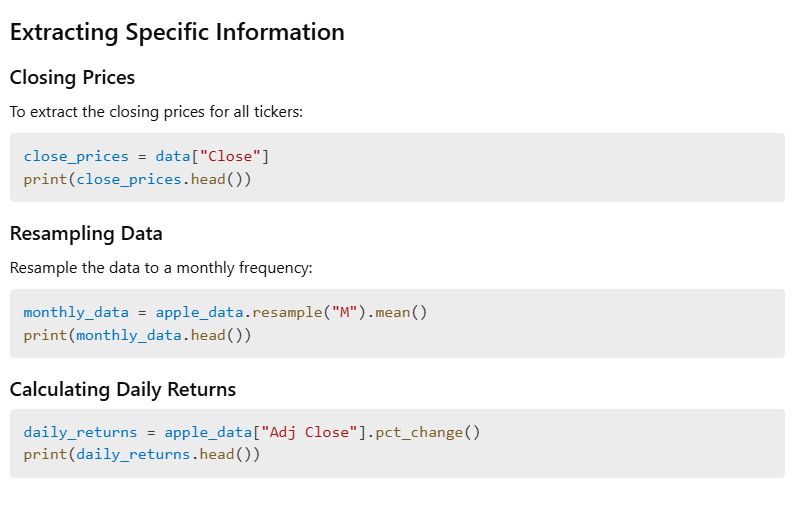
\includegraphics[scale=0.55]{../05-pictures/lesson-1-3_pic_16.png}
	\end{center}
\end{frame}
%..................................................................
\begin{frame}{Data Gathering with Pandas}
	\begin{center}
	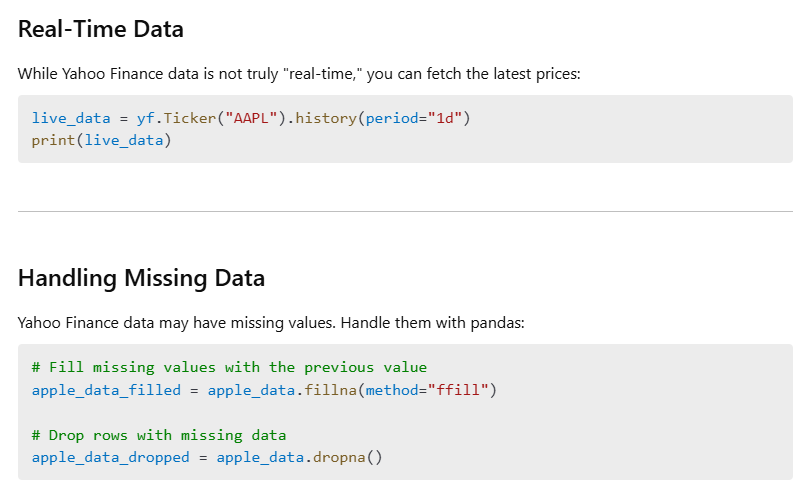
\includegraphics[scale=0.55]{../05-pictures/lesson-1-3_pic_17.png}
	\end{center}
\end{frame}
%..................................................................
\begin{frame}{Data Gathering with Pandas}
	\begin{center}
	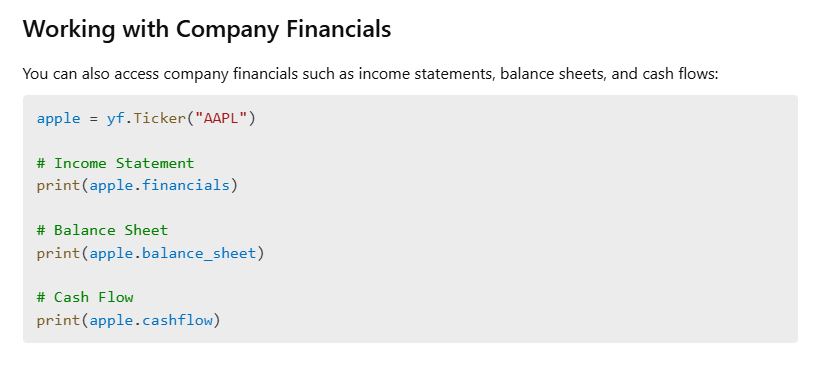
\includegraphics[scale=0.55]{../05-pictures/lesson-1-3_pic_18.png}
	\end{center}
\end{frame}
%..................................................................
\begin{frame}{Data Gathering with Pandas}
	\begin{center}
	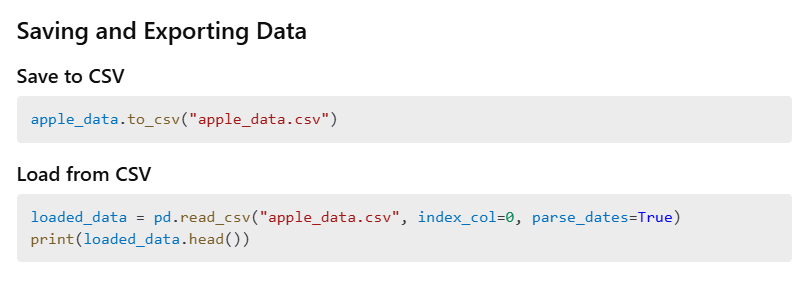
\includegraphics[scale=0.55]{../05-pictures/lesson-1-3_pic_19.png}
	\end{center}
\end{frame}
%..................................................................
%=====================================================================


\end{document}
